This section follows up from the design described in \cref{sec:sprint3:designsettings}.
When clicking the ''Apps'' pane, the fragment filled into the fragment container in \lstinline!SettingsActivity! is \lstinline!AppManagementFragment!.
\lstinline!AppManagementFragment! in turn contains another fragment container, \lstinline!AppsContainer!, where the two fragments derived from \lstinline!AppContainerFragment! will be loaded in - the fragments showing the applications.
Furthermore, \lstinline!AppContainerFragment! implements three buttons in the top of the layout:

\begin{itemize}
\item The \textbf{Giraf} button loads the \lstinline!GirafFragment! into the fragment container
\item The \textbf{Android} button loads the \lstinline!AndroidFragment! into the fragment container
\item The \textbf{Google Play} button opens the Play Store App. If the apps is not installed on the device, it opens the Play Store in the default browser.
\end{itemize}

The \textbf{Giraf} button and the \textbf{Android} button loads a new fragment into \lstinline!AppsContainer!, by using a \lstinline!FragmentManager!
An  \lstinline!OnClickListener! is attached to the \textbf{Giraf} and \textbf{Android} buttons, which call the method \lstinline!replaceFragment()!, sending the appropriate fragment as argument to \lstinline!replaceFragment()!.
The method \lstinline!replaceFragment()! can be seen in \cref{lst:replaceFragment}.

\begin{lstlisting}[caption={Method used to replace the fragment currently loaded into the fragment container in AppManagementFragment}, label={lst:replaceFragment}]
/**
 * Replace active fragment by running the transaction in a new thread.
 * Adds responsiveness when loading list of installed apps_container.
 * @param fragment
 */
private void replaceFragment(final Fragment fragment){
    new Runnable() {
        @Override
        public void run() {
            FragmentTransaction ft = fragmentManager.beginTransaction();
            ft.replace(R.id.app_settings_fragmentlayout, fragment);
            ft.commit();
        }
    }.run();
}
\end{lstlisting}

The \textbf{Google Play} button opens the Google Play Store, so the user can download additional Android applications, if desired. 
Firstly, we researched how to use the inbuilt API for Google Services  to open the Play Store in this way.
However, there were some problems with the API when attempting to implement.
Furthermore, it was discovered that the API is intended to be used for syncronization with Google+, Google Drive and Google Games.
Therefore, we ultimately chose to open the Play Store as a separate activity with the \lstinline!Intent.FLAG_ACTIVITY_NEW_TASK! and the \lstinline!Intent.FLAG_ACTIVITY_CLEAR_TOP! flags.
The exact code can be seen in \cref{lst:launchergoogleplay}.\vagner{Please read this and refactor it.}

The full design can be seen visualized in \cref{fig:settingsappfragments}.
 
\begin{figure}[h]
\centering
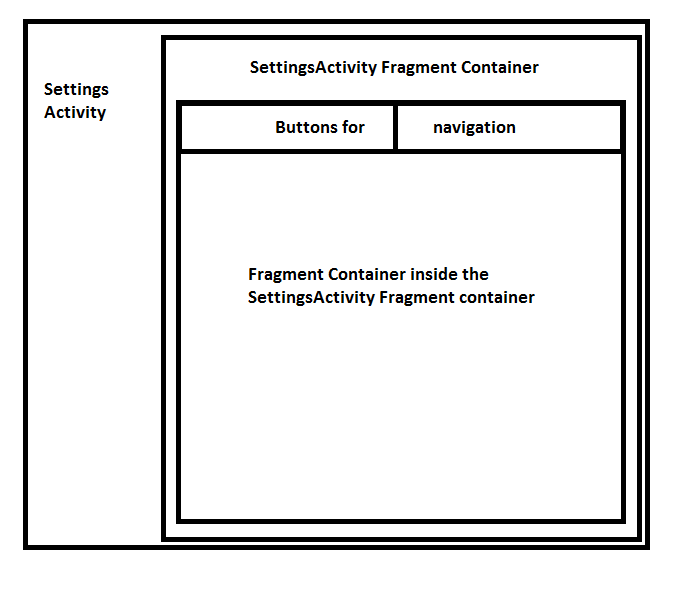
\includegraphics[width=\textwidth, height=3in, keepaspectratio=true] {SettingsActivity.png}
\caption{The organization of \lstinline!SettingsActivity! when inside the "Apps" pane. Since we need to distinguish between \giraf and Android applications, nested fragment containers are used.}
\label{fig:settingsappfragments}
\end{figure}

\paragraph{AppContainerFragment and the derived classes}

Because the \giraf and Android fragments contain many of the same variables, these inherit all shared information from a superclass, consequently reducing redundancy and clarifying how the two fragments are different.
This superclass is called \lstinline!AppManagementFragment! and the main responsibilities are:

\begin{itemize}
\item Initialize shared variable in \lstinline!onCreate()!
\item Implement shared methods handling when to load applications
\end{itemize}

As a result, the two derived classes get their shared variables initialized by a call to \lstinline!super.onCreate()! and reloading of applications is handled automatically by \lstinline!AppContainerFragment!. \\

However, which type of apps are loaded where different between \lstinline!AndroidFragment! and \lstinline!GirafFragment!.
As noted in \cref{sec:sprint:designlauncher} and explained in \cref{sect:sprint3:refactoring}, the functions used to load applications into view was moved from \lstinline!HomeActivity! to \lstinline!LauncherUtility!.
This was solved by initializing the shared variable \lstinline!apps! differently in the two derived classes -
\lstinline!GirafFragment! loaded \giraf applications into \lstinline!apps!, while \lstinline!AndroidFragment! loaded Android applications into it.

Since the automatic load methods mentioned above work on the \lstinline!apps! variable, this solution solved the problem. \\

However, one problem has to be directly inside the two derived classes, namely marking the applications as selected and adding them to the users list of selected applications.
This is due to the fact that \giraf applications are saved as the \textit{OasisLib} type \lstinline!Application!, while Android applications are saved as the type \lstinline!ResolveInfo!.

The \giraf applications connected to a user are saved or removed through a call to an \textit{OasisLib} method, as can be seen in \cref{lst:addinggirafapplications}.

\begin{lstlisting}[caption={The methods used for adding or removing a Giraf application to a user}, label={lst:addinggirafapplications}]
ProfileApplicationController pac = new ProfileApplicationController(context);
ProfileApplication pa = new ProfileApplication(currentUser.getId(), app.getApp().getId());
if(pa == null)
	pac.insertProfileApplication(pa);
else
	pac.removeProfileApplicationByProfileAndApplication(app.getApp(), currentUser);
\end{lstlisting}

Android applications are saved as a file containing \lstinline!Set<String>!, stored in the native \lstinline!SharedPreferences! of Android.
Each file name is made, unique to each user, by incorporating the users ID as part of the file name.
More about saving settings in Android can be found in \cref{para:sprint4:managingsettingsandroid}.
The code can be seen in \cref{lst:addingandroidapplications}\\

\begin{lstlisting}[caption={The methods used for adding or removing a GIRAF application to a user. Please note that the documentation has been removed.}, label={lst:addingandroidapplications}]
String activityName = app.getActivity();

if (selectedApps.contains(activityName))
    selectedApps.remove(activityName);
else
    selectedApps.add(activityName);
\end{lstlisting}

This also means that the two fragments must handle the selected applications different, when marking them the first time a fragment is loaded.
The code is not included, since it is similar to that of \cref{lst:addinggirafapplications} and \cref{lst:addingandroidapplications} - the same checks are carried out, but rather than being for a single application, they are carried out on all installed applications.